\documentclass[10pt, a4paper]{article}

% \usepackage{fullpage}
\usepackage[margin=1in]{geometry}
% \usepackage[top=1in, bottom=1in, left=0.75in, right=0.75in, paperwidth=5in, paperheight=7in]{geometry}
\usepackage{amsfonts, amssymb, amsmath}
\usepackage{tikz, pgfplots} %für das Taschenrechner Icon
\usepackage{graphicx} %für das einbinden von Bildern
\usepackage{float} %benötigt f+r \begin{figure}[H<--]

% \usepackage{tgbonum} %font family TEX Gyre Bonum
\usepackage{helvet}

\def\eq1{y=\frac{x}{3x^2+x+1}}

\newcommand{\set}[1]{\setlength\itemsep{#1em}}
\newcommand{\blank}[1]{\line(1,0){#1}\,}
\newcommand\calculator{\tikz{
		\node (c) [inner sep=0pt, draw, fill=black, anchor=south west]{\phantom{N}};
		\begin{scope}[x=(c.south east),y=(c.north west)]    \fill[white] (.1,.7) rectangle (.9,.9);    
		\foreach \x in {.1, .33, .55, .79}{    
		\foreach \y in {.1, .24, .38, .53}{    
		\fill[white] (\x,\y) rectangle + (.11,.07);}} 
		\end{scope} }}
		\def\calcicon#1{\noindent#1 \calculator\ }
        \pgfplotsset{compat=1.18}
\begin{document}

\textbf{Critical Thinking Questions}

% 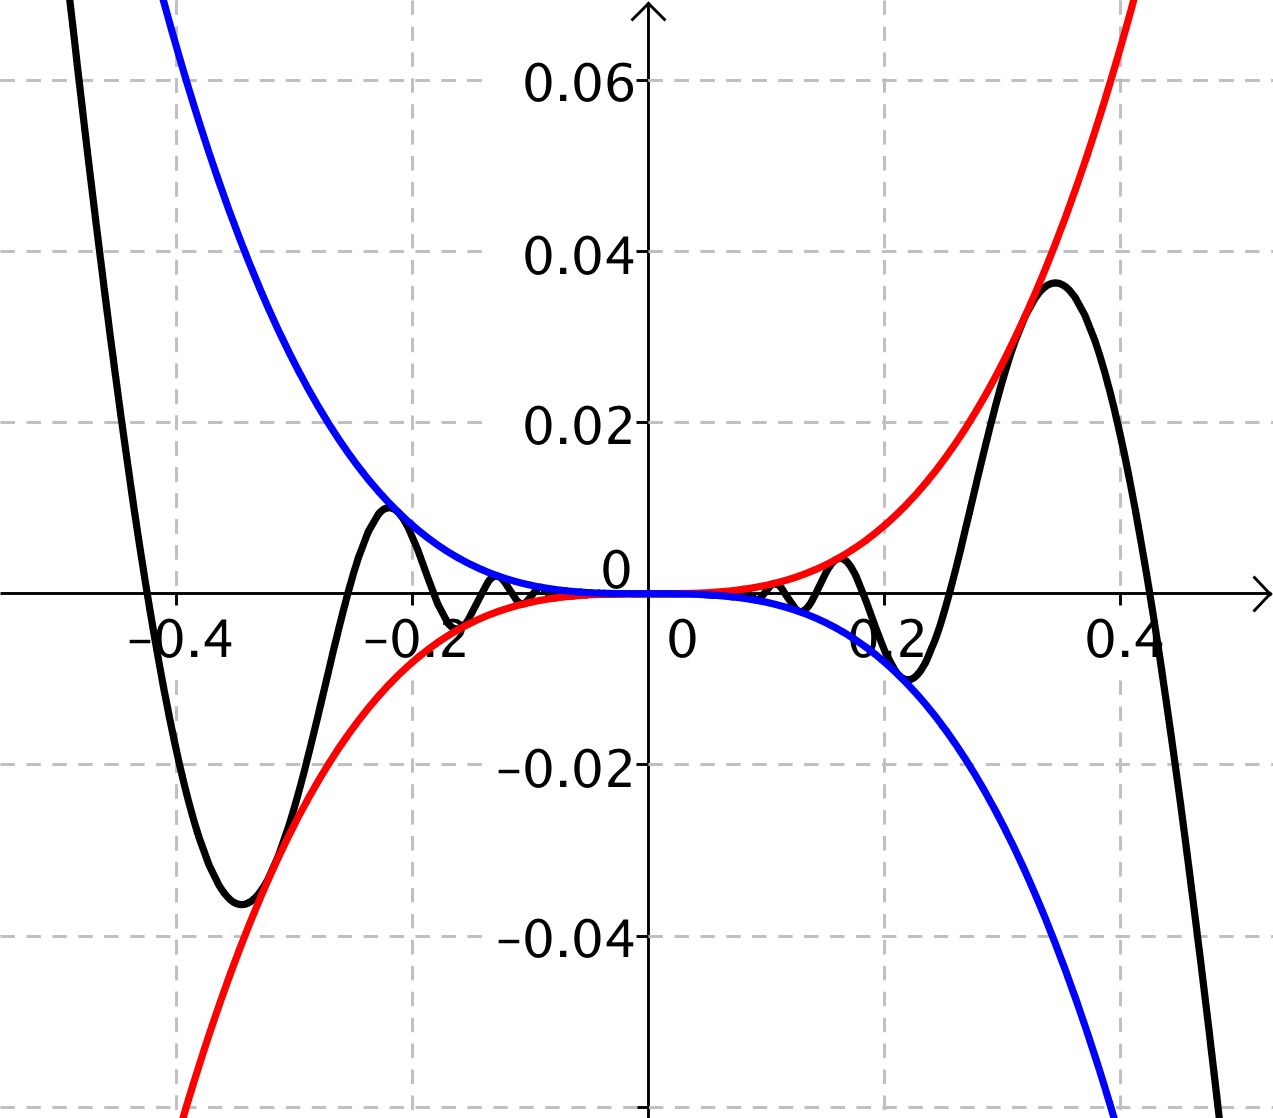
\includegraphics[scale=0.6]{Tutorial Shared Files/Old Tutorials/limit}
\begin{figure}[H]
    \centering
    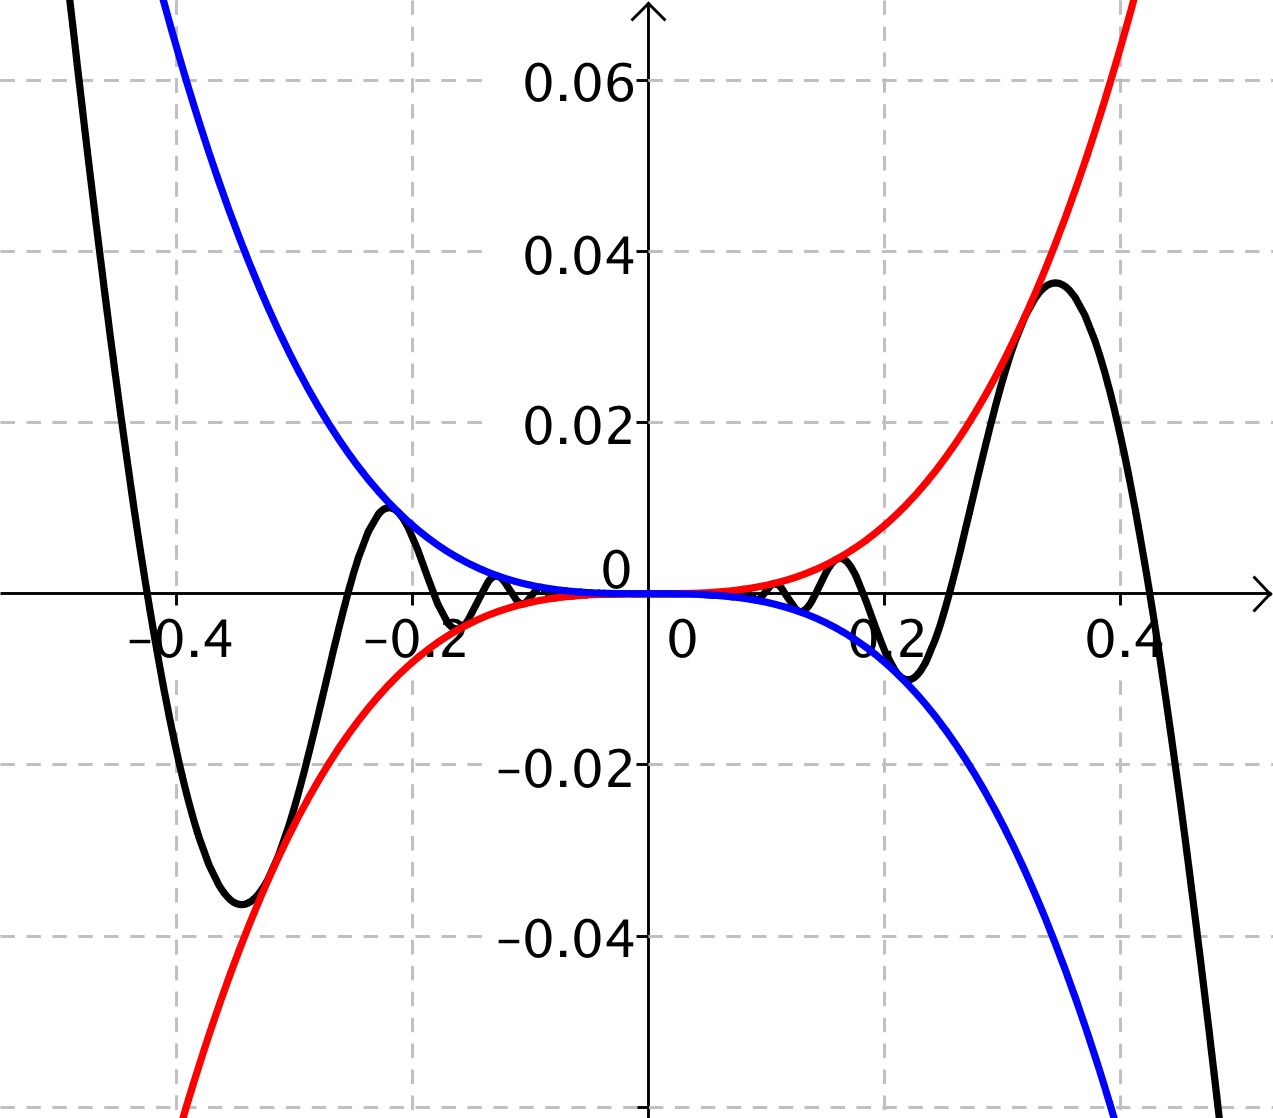
\includegraphics[width=0.4\textwidth]{Tutorial Shared Files/Old Tutorials/limit}
    \caption{The Squeeze Theorem}
\end{figure}

\begin{enumerate}
    \set{1.2}
    \item \calculator\ Let's examine the function \(\eq1\).
    \item \textsf{This} is the symbol for the set of all real numbers: $\mathbb{R}$.
    \item This is the symbol for the set of integer: $\mathbb{Z}$.
    \item This is the symbol for the set of rational numbers: $\mathbb{Q}$.
    \item Is it possible for a sequence to converge to two different numbers? If so, give an example. If not, explain why not.
    \item Explain how to use partial sums to determine if a series converges or diverges. Give an example
    \item Explain why \(\int\limits_{1}^{\infty} f(x)\,dx\) and $\sum\limits_{n=1}^{\infty} a_n$ need not converge to the same value, even if they are both convergent.
    \item In your own words, explain the Alternating Series Remainder Theorem. How is this theorem useful?
    \item Explain the difference between absolute and conditional convergence. Give an example of each.
    \item The Ratio Test is in conclusive if $\lim\limits_{n\rightarrow\infty} \left|\frac{a_{n+1}}{a_n}\right|=1$. Give an example of one convergent series and one divergent series for which $\lim\limits_{n\rightarrow\infty} \left|\frac{a_{n+1}}{a_n}\right|=1$. Explain how you determined your examples.
\end{enumerate}

\end{document}